% Provenance (never printed): see sources/outline_sources.md (Year 2: fractional
% crystallisation, Bowen's series, compatible and incompatible elements, mixing and
% assimilation, layered intrusions).
% Curves from figdata/bachelor-2/differentiation.py (Bowen 1913 plagioclase loop, Rayleigh and
% equilibrium laws, Wilcox 1954 Paricutin analyses and mass balance, AFC closed form,
% Tegner et al. 2023 Skaergaard whole-rock data); exercise and problem values in the Book 4
% scratch calculator calc/ch08.py.
\chapter{التمايز الصهاري}\label{ch:b2:magmatic-differentiation}

في 20 فبراير 1943 بدأ بركان يثور في غرب المكسيك، ودام ثورانه
تسع سنوات. كانت حممه الأولى أنديزيتًا بازلتيًا فيه \qty{55}{\percent} من
السيليكا؛ وكانت حممه الأخيرة، في فبراير 1952، أنديزيتًا فيه أكثر بقليل من
\qty{60}{\percent}. ولم ينتقل البركان، باريكوتين، إلى مصدر آخر في
أثناء ذلك، وحُلّلت حممه واحدة بعد أخرى كلما خرجت. \omterm{def:b2:magma-emplacement:magma}{فالصهارة}
تحته هي التي غيّرت نفسها: أنمت بلورات وتركتها خلفها، والتهمت
شيئًا من الصخر الغرانيتي المحيط بها. \omterm{def:b2:magma-emplacement:magma}{والصهارة} التي تغادر الوشاح بازلتًا قد
تنتهي ريوليتًا، والصخور التي تخلّفها في طريقها تسجّل كيف حدث ذلك.
يتتبّع هذا الفصل صهارة وهي تبرد: الترتيب الذي تتبلور به المعادن،
والقوانين التي تبيّن كيف تتغيّر العناصر الرئيسية والنزرة حين تُزال البلورات،
والصخور المبنيّة من تلك البلورات، وما يحدث حين تتلقّى \omterm{def:b2:magma-emplacement:magma}{الصهارة}
صهارة أخرى أو تبتلع القشرة.
% ledger: wilcox54:paricutin

\begin{recall}
\textbf{من مجلد المرحلة الثانوية}: الصخور النارية ونسجها؛ والترتيب
الذي تتبلور به المعادن من صهارة بازلتية، الأوليفين أولًا والكوارتز أخيرًا،
كما وجدته تجارب بوين. \textbf{من مجلد السنة الثانية من كتب الكيمياء}:
مخطّطات الأطوار الثنائية، والمحاليل الصلبة وقاعدة الرافعة. \textbf{من مجلد السنة
الأولى}: البلاجيوكليز، وهو محلول صلب بين الأنورثيت \ce{CaAl2Si2O8}
والألبيت \ce{NaAlSi3O8}، والسيليكات الأخرى المكوّنة للصخور؛ والشرائح الرقيقة بين
مستقطِبين متعامدين. \textbf{من \cref{ch:b2:elements-in-the-earth}}: معاملات التوزيع بين المعدن والمصهور
ومعاملات التوزيع الكلية، $\bar D = \sum_i x_i D_i$، والعناصر المتوافقة وغير المتوافقة،
\omterm{def:b2:elements-in-the-earth:normalised}{والمخطّطات المعايَرة} \omterm{prop:b2:elements-in-the-earth:normalised}{وشذوذ اليوروبيوم}. \textbf{من
\cref{ch:b2:isotope-geochemistry}}: النسب النظائرية مقتفياتٍ، والقطع
الزائد للمزج. \textbf{من \cref{ch:b2:mantle-melting}}: أوتكتيك الديوبسيد--الأنورثيت،
\omterm{def:b2:mantle-melting:peritectic}{والانصهار غير المتطابق}، والمخطّطات الثلاثية، والصهارات الأولية.
\end{recall}

\section{تتابعات التبلور}\label{sec:b2:magmatic-differentiation:sequences}

لا تبلور \omterm{def:b2:magma-emplacement:magma}{الصهارة} البازلتية كل معادنها دفعة واحدة. فقد وجد بوين
بالتجربة أن الأوليفين يتبلور أولًا في العادة، بين 1200
و\qty{1300}{\celsius}؛ وأن البلاجيوكليز الغني بالكالسيوم يبدأ قرابة حيث يبدأ
البيروكسين؛ وأن آخر سائل، الغني بالسيليكا، يعطي فلسبار البوتاسيوم والكوارتز
وربما المسكوفيت عند نحو 750 إلى \qty{800}{\celsius}. وبين الطرفين لا تتراكم
المعادن المافية ببساطة: بل يتفاعل كل منها مع السائل ليعطي التالي.
% ledger: earle:bowen (Book 2), tulane:bowen (Book 2)

\begin{definition}[سلسلة بوين التفاعلية]\label{def:b2:magmatic-differentiation:bowen}
\emph{سلسلة بوين التفاعلية}\index{سلسلة بوين التفاعلية} هي الترتيب الذي
تتبلور به السيليكات الشائعة من صهارة بازلتية تبرد، في فرعين
يلتقيان في النهاية. ففي \emph{الفرع غير المستمر} يتفاعل كل معدن مافي
مع السائل ليكوّن معدنًا جديدًا ذا بنية أخرى: الأوليفين،
فالبيروكسين، فالأمفيبول، فالبيوتيت. وفي \emph{الفرع المستمر} يتبلور البلاجيوكليز
على طول الطريق، ويتغيّر تركيبه باستمرار من الغني بالكالسيوم
إلى الغني بالصوديوم. ويبلور آخر سائل فلسبار البوتاسيوم والمسكوفيت
والكوارتز.
\end{definition}
% ledger: earle:bowen (Book 2)

\begin{omfigure}
\centering
\begin{tikzpicture}[font=\small, x=1cm, y=1cm,
  mn/.style={draw, rounded corners=2pt, fill=white, inner sep=3pt, minimum width=2.3cm,
             align=center}]
\draw[-{Stealth[length=4pt]}, thick, gray] (-1.3,0.3) -- (-1.3,-6.0);
\node[rotate=90, anchor=south, font=\scriptsize, gray] at (-1.4,-2.85) {درجة حرارة متناقصة};
\node[anchor=east, font=\scriptsize] at (-1.5,0) {$\approx$ 1200--\qty{1300}{\celsius}};
\node[anchor=east, font=\scriptsize] at (-1.5,-5.6) {$\approx$ 750--\qty{800}{\celsius}};
\node[mn] (ol) at (1,0) {أوليفين};
\node[mn] (px) at (1,-1.4) {بيروكسين};
\node[mn] (am) at (1,-2.8) {أمفيبول};
\node[mn] (bt) at (1,-4.2) {بيوتيت};
\draw[-{Stealth[length=4pt]}, thick] (ol) -- (px);
\draw[-{Stealth[length=4pt]}, thick] (px) -- (am);
\draw[-{Stealth[length=4pt]}, thick] (am) -- (bt);
\node[font=\scriptsize, align=center] at (1,0.8) {الفرع غير المستمر\\\foreignlanguage{arabic}{(معدن جديد عند كل خطوة)}};
\node[mn] (ca) at (6,-1.4) {بلاجيوكليز\\غني بالكالسيوم};
\node[mn] (na) at (6,-4.2) {بلاجيوكليز\\غني بالصوديوم};
\fill[left color=white, right color=white, top color=orange!35, bottom color=orange!8]
  (5.75,-2.0) rectangle (6.25,-3.6);
\draw[-{Stealth[length=4pt]}, thick] (ca) -- (na);
\node[font=\scriptsize, align=center] at (6,0.8) {الفرع المستمر\\\foreignlanguage{arabic}{(معدن واحد يتغيّر تركيبه)}};
\node[mn, minimum width=7.2cm] (last) at (3.5,-5.6) {\foreignlanguage{arabic}{فلسبار البوتاسيوم، المسكوفيت، الكوارتز}};
\draw[-{Stealth[length=4pt]}, thick] (bt) -- (bt|-last.north);
\draw[-{Stealth[length=4pt]}, thick] (na) -- (na|-last.north);
\end{tikzpicture}
\par\smallskip{\small \omterm{def:b2:magmatic-differentiation:bowen}{سلسلة بوين التفاعلية}. يتبلور الأوليفين والبلاجيوكليز الغني بالكالسيوم
أولًا من صهارة بازلتية؛ وفي الجهة اليسرى يتفاعل كل معدن مافي مع
السائل ليعطي التالي، وفي الجهة اليمنى يزداد البلاجيوكليز غنًى
بالصوديوم؛ ويعطي آخر سائل، الغني بالسيليكا، فلسبار البوتاسيوم والمسكوفيت والكوارتز.
ودرجات الحرارة قيم نموذجية لصهارة بازلتية عند ضغط منخفض.}
\end{omfigure}
% ledger: earle:bowen (Book 2)

يقابل الفرعان نوعي مخطّطات الأطوار في
\cref{ch:b2:mantle-melting}. فالتفاعل غير المستمر هو \omterm{def:b2:mantle-melting:peritectic}{الانصهار غير المتطابق}
للإنستاتيت معكوسًا: تتفاعل بلورات الفورستريت مع سائل أغنى بالسيليكا لتعطي
الإنستاتيت. والفرع المستمر محلول صلب. وقد قاسه بوين عام 1913
على بلاجيوكليزات صناعية، فأبقى كل تركيب عند درجة حرارة معلومة
وبحث عن الزجاج والبلّورات: ينصهر الأنورثيت عند \qty{1550}{\celsius}، والألبيت عند
نحو \qty{1100}{\celsius}، وكل بلاجيوكليز وسيط ينصهر على مجال
بين منحنى أدنى، هو خط الصلابة، ومنحنى أعلى، هو خط السيولة (الشكل
أدناه).
% ledger: bowen13:plagioclase, bowen14:mgo-sio2

\begin{omfigure}
\centering
\begin{tikzpicture}
\begin{axis}[omrecord, width=0.78\linewidth, height=6.4cm,
  xmin=0, xmax=100, ymin=1050, ymax=1600,
  xlabel={\foreignlanguage{arabic}{الأنورثيت \babelsublr{(\unit{\percent})} جزيئيًا}}, ylabel={\foreignlanguage{arabic}{درجة الحرارة \babelsublr{(\unit{\celsius})}}},
  y tick label style={/pgf/number format/1000 sep={}}, unbounded coords=discard,
  tick label style={font=\scriptsize}, label style={font=\small}]
\addplot[very thick, black] table[x=an, y=T_liq] {figdata/out/bachelor-2-differentiation-plag-curve.dat};
\addplot[very thick, black, dashed] table[x=an, y=T_sol] {figdata/out/bachelor-2-differentiation-plag-curve.dat};
\addplot[only marks, mark=*, mark size=1.5pt, blue!70!black] table[x=an, y=T_liq] {figdata/out/bachelor-2-differentiation-plag-data.dat};
\addplot[only marks, mark=o, mark size=1.7pt, blue!70!black] table[x=an, y=T_sol] {figdata/out/bachelor-2-differentiation-plag-data.dat};
\draw[densely dotted, red!70!black, thick] (axis cs:50,1560) -- (axis cs:50,1287);
\draw[red!70!black, thick] (axis cs:50,1450) -- (axis cs:80.6,1450);
\draw[red!70!black, thick] (axis cs:33.3,1394) -- (axis cs:70.6,1394);
\draw[red!70!black, thick] (axis cs:13.9,1287) -- (axis cs:50,1287);
\addplot[only marks, mark=*, mark size=1.4pt, red!70!black] coordinates {(50,1450) (80.6,1450) (33.3,1394) (70.6,1394) (13.9,1287) (50,1287)};
\node[font=\scriptsize] at (axis cs:30,1530) {سائل};
\node[font=\scriptsize, align=center] at (axis cs:83,1200) {بلاجيوكليز\\\foreignlanguage{arabic}{(محلول صلب)}};
\node[font=\scriptsize, anchor=west] at (axis cs:2,1430) {\foreignlanguage{arabic}{خط السيولة (الخط المتصل)}};
\node[font=\scriptsize, anchor=west] at (axis cs:42,1160) {\foreignlanguage{arabic}{خط الصلابة (المتقطّع)}};
\node[font=\scriptsize, anchor=south, red!70!black, fill=white, inner sep=1pt] at (axis cs:68,1452) {\qty{1450}{\celsius}};
\node[font=\scriptsize, anchor=north, red!70!black, fill=white, inner sep=1pt] at (axis cs:31,1284) {\qty{1287}{\celsius}};
\end{axis}
\end{tikzpicture}
\par\smallskip{\small البلاجيوكليزات الفلسبارية عند الضغط الجوي، من
تجارب السقي لبوين (1913): بداية الانصهار (الدوائر) واكتماله (النقاط)،
مع منحنيات مرسومة عبر القياسات. وبالأحمر، \omterm{def:b2:magmatic-differentiation:crystallisation}{التبلور المتوازن}
لسائل فيه \qty{50}{\percent} من الأنورثيت: أول بلّورة، عند
\qty{1450}{\celsius}، فيها \qty{81}{\percent} من الأنورثيت؛ وعند \qty{1394}{\celsius}
تتعايش بلّورات فيها \qty{71}{\percent} مع سائل فيه \qty{33}{\percent}؛ وآخر
سائل، عند \qty{1287}{\celsius}، فيه \qty{14}{\percent} (\cref{exo:b2:magmatic-differentiation:1}).}
\end{omfigure}
% ledger: bowen13:plagioclase

السائل الذي يبلور محلولًا صلبًا يغتني بالمكوّن الذي
ينصهر عند درجة الحرارة الأدنى: فأول بلاجيوكليز من سائل فيه
\qty{50}{\percent} من الأنورثيت فيه \qty{81}{\percent}، ويتحرّك السائل نحو
الألبيت. وما يحدث بعد ذلك يتوقّف على بقاء البلّورات في حوار مع
السائل أو عدمه.

\begin{definition}[التبلور المتوازن والتبلور التجزيئي]
\label{def:b2:magmatic-differentiation:crystallisation}
في \emph{التبلور المتوازن}\index{التبلور المتوازن} تبقى
البلّورات في توازن كيميائي مع السائل كله حتى
النهاية، وتعيد توازنها كلما تغيّر السائل؛ فينتهي النظام بالتركيب
الذي بدأ به. وفي \emph{التبلور التجزيئي}\index{التبلور التجزيئي} تُعزل كل بلّورة، بمجرّد تكوّنها، عن التفاعل مع
السائل، بالترسّب، أو بالالتصاق بجدران الحجرة، أو بأن
يغلّفها نموّ لاحق؛ فيتطوّر السائل عندئذ كأن البلّورات قد
أُخرجت من النظام.
\end{definition}

في \omterm{def:b2:magmatic-differentiation:crystallisation}{التبلور المتوازن} يتغيّر بلاجيوكليز الشكل أعلاه من
\qty{81}{\percent} إلى \qty{50}{\percent} من الأنورثيت وهو ينمو، إذ تعيد كل بلّورة
توازنها بالانتشار مع السائل، ويختفي آخر سائل عند
خط الصلابة، \qty{1287}{\celsius}. لكن الانتشار في الفلسبار بطيء،
وقلّما تجاري البلّورات الطبيعية ذلك: فداخل كل بلّورة ينقطع عن السائل،
الذي يسلك عندئذ كما في \omterm{def:b2:magmatic-differentiation:crystallisation}{التبلور التجزيئي} ويمكن أن يبلغ تراكيب
قريبة من الألبيت. ويحسب الشكل في القسم الأخير من هذا الفصل المسارين كليهما.
% ledger: bowen13:plagioclase

\begin{definition}[خط النزول السائل]\label{def:b2:magmatic-differentiation:lld}
\emph{خط النزول السائل}\index{خط النزول السائل} لصهارة هو
تتابع التراكيب التي يتّخذها سائلها وهو يتبلور، مرسومةً على
مخطّط تغيّر أو مخطّط أطوار.
\end{definition}

\omterm{def:b2:magmatic-differentiation:lld}{خط النزول السائل} خاصية للسائل وحده. فالحمم التي تثور وفيها
بلّورات لا تقع عليه تمامًا، ولذلك استعمل ويلكوكس، في دراسته حمم
باريكوتين، تحاليل الصخر الكلي وتراكيب
أرضيتها، أي الجزء السائل، محسوبةً بإزالة البلّورات.
% ledger: wilcox54:groundmass

\section{التبلور التجزيئي للعناصر الرئيسية}\label{sec:b2:magmatic-differentiation:majors}

إزالة البلّورات تغيّر تركيب السائل على نحو بسيط وخطي،
وأقدم أداة لقراءته هي رسم كل أكسيد بدلالة السيليكا.

\begin{definition}[مخطّط هاركر]\label{def:b2:magmatic-differentiation:harker}
\emph{مخطّط هاركر}\index{مخطّط هاركر} (مخطّط التغيّر بدلالة السيليكا) يرسم
النسبة المئوية الكتلية لكل أكسيد في متتالية من الصخور المترابطة بدلالة نسبتها
المئوية الكتلية من \ce{SiO2}، بلوحة لكل أكسيد.
\end{definition}


تُظهر حمم باريكوتين اتجاهات كهذه (\omterm{def:b2:magmatic-differentiation:harker}{مخطّطات هاركر} بعد القضية
التالية): فمع ارتفاع السيليكا تنخفض المغنيسيا والجير والألومينا ويرتفع البوتاس. وهذا
ما تفعله إزالة الأوليفين والبلاجيوكليز:
فالأوليفين يأخذ المغنيسيا والحديد، والبلاجيوكليز الجير والألومينا، وكلاهما يترك
السائل أغنى بالسيليكا والقلويات. أمّا هل تستطيع إزالة معادن معروفة أن
تفسّر الاتجاهات كمّيًا، فتلك مسألة موازنة كتلية.

\begin{proposition}[الموازنة الكتلية لإزالة البلّورات]\label{prop:b2:magmatic-differentiation:lever}
لتكن صهارة أمّ تركيبها $\mathbf p$ (متّجه الكسور الكتلية للأكاسيد)
تبلور معادن تراكيبها $\mathbf m_1, \dots, \mathbf m_k$ بكتل
$x_1, \dots, x_k$ لكل وحدة كتلة من الأمّ، وليكن $\mathbf d$ تركيب
السائل المتبقّي. عندئذ
\[
\mathbf p = \Big(1 - \sum_i x_i\Big)\mathbf d + \sum_i x_i \mathbf m_i .
\]
ومن أجل معدن واحد، تقع الأمّ على القطعة المستقيمة الواصلة بين السائل
والمعدن في كل مخطّط تغيّر، والكسر الكتلي المُزال هو
$x = (p_j - d_j)/(m_j - d_j)$ لأيّ أكسيد $j$: إنها قاعدة الرافعة.
\end{proposition}

\begin{proof}
كل أكسيد محفوظ: فالكتلة $p_j$ من الأكسيد $j$ في وحدة كتلة من الأمّ تنتهي
إمّا في السائل، الذي كتلته $1 - \sum_i x_i$ وتركيزه $d_j$، وإمّا في
المعادن. وكتابة ذلك لكل $j$ تعطي المعادلة المتّجهة. ومع معدن واحد
تصبح $\mathbf p = (1-x)\mathbf d + x\mathbf m$، أي نقطة من القطعة الممتدّة من
$\mathbf d$ إلى $\mathbf m$ تقسمها بالنسبة $x : (1-x)$، على أيّ زوج من
المحاور؛ وحلّ مركّبة واحدة يعطي $x$.
\end{proof}

\begin{omfigure}
\centering
\begin{tikzpicture}
\begin{groupplot}[group style={group size=2 by 2, horizontal sep=1.6cm, vertical sep=1.3cm},
  width=0.44\linewidth, height=4.3cm, omrecord, xmin=54.5, xmax=60.8,
  tick label style={font=\scriptsize}, label style={font=\small},
  xtick={55,56,57,58,59,60}]
\nextgroupplot[ylabel={\mbox{\textdir TLT \ce{MgO} (\unit{\percent})}}, ymin=3.2, ymax=6.0]
\addplot[only marks, mark=*, mark size=1.3pt, blue!70!black] table[x=SiO2, y=MgO] {figdata/out/bachelor-2-differentiation-paricutin.dat};
\nextgroupplot[ylabel={\mbox{\textdir TLT \ce{CaO} (\unit{\percent})}}, ymin=6.0, ymax=7.6]
\addplot[only marks, mark=*, mark size=1.3pt, blue!70!black] table[x=SiO2, y=CaO] {figdata/out/bachelor-2-differentiation-paricutin.dat};
\nextgroupplot[ylabel={\mbox{\textdir TLT \ce{K2O} (\unit{\percent})}}, ymin=0.7, ymax=1.9, xlabel={\mbox{\textdir TLT \ce{SiO2} (\unit{\percent})}}]
\addplot[only marks, mark=*, mark size=1.3pt, blue!70!black] table[x=SiO2, y=K2O] {figdata/out/bachelor-2-differentiation-paricutin.dat};
\node[font=\scriptsize, anchor=west] at (axis cs:55.1,0.80) {1943};
\node[font=\scriptsize, anchor=east] at (axis cs:60.0,1.82) {1952};
\nextgroupplot[ylabel={\mbox{\textdir TLT \ce{Al2O3} (\unit{\percent})}}, ymin=17.0, ymax=19.0, xlabel={\mbox{\textdir TLT \ce{SiO2} (\unit{\percent})}}]
\addplot[only marks, mark=*, mark size=1.3pt, blue!70!black] table[x=SiO2, y=Al2O3] {figdata/out/bachelor-2-differentiation-paricutin.dat};
\end{groupplot}
\end{tikzpicture}
\par\smallskip{\small \omterm{def:b2:magmatic-differentiation:harker}{مخطّطات هاركر} لحمم باريكوتين التي حلّلها
ويلكوكس (1954)، وعددها 22، وقد ثارت من فبراير 1943 (أدنى سيليكا) إلى فبراير 1952. فمع
ارتفاع السيليكا بخمسة في المئة تنخفض المغنيسيا والجير والألومينا ويكاد البوتاس
يتضاعف.}
\end{omfigure}
% ledger: wilcox54:table2, wilcox54:paricutin

مع عدّة معادن تُوجد الكتل بحلّ معادلات الحفظ لعدد مماثل
من الأكاسيد. وقد فعل ويلكوكس ذلك بيانيًا عام 1954؛ وهو اليوم نظام خطي
صغير.

\begin{method}[الموازنة الكتلية بالمربعات الصغرى]\label{met:b2:magmatic-differentiation:massbalance}
لاختبار ما إذا كان سائل وليد $\mathbf d$ مشتقًا من أمّ $\mathbf p$ بإزالة
المعادن $\mathbf m_1, \dots, \mathbf m_k$ (وبإضافة صخر
مُستوعَب عند الحاجة، يُدخَل بكتلة سالبة): (1) لكل أكسيد $j$، اكتب
حفظ القضية بعد إعادة ترتيبه معادلةً خطية في الكتل
المُزالة لكل \qty{100}{g} من الأمّ،
\[
\sum_i x_i\,(m_{ij} - d_j) = 100\,(p_j - d_j);
\]
(2) مع $k$ أكسيدًا بالضبط، تُختار من بين ما تغيّره المعادن أكثر، حلّ
النظام $k \times k$؛ ومع أكاسيد أكثر، حلّه بالمربعات الصغرى (صغّر مجموع
مربعات الفروق بين الطرفين)؛ (3) أعد حساب الوليد من
الكتل الموجودة وقارنه بالتحليل، أكسيدًا أكسيدًا: فالبواقي الأكبر
من أخطاء التحليل، أو كتلة سالبة لمعدن، ترفض النموذج.
\end{method}

اختار ويلكوكس السيليكا والألومينا والمغنيسيا ضوابطه الثلاثة، وثلاث
مواد: أوليفين تركيبه Fo$_{80}$، وبلاجيوكليز An$_{70}$، ومتوسط
أربعة صخور دخيلة غرانيتية (\qty{72.5}{\percent} من \ce{SiO2}، و\qty{3.6}{\percent} من
\ce{K2O}) وُجدت في الحمم. وبيّن أن لا تركيبة من الأوليفين
والبلاجيوكليز وحدهما تلائم المتتالية، وأن إضافة \qty{25.4}{g} من الصخر الدخيل
وإزالة \qty{2.9}{g} من الأوليفين و\qty{9.6}{g} من البلاجيوكليز من
\qty{100}{g} من أرضية الحمم الأولى تعطي \qty{112.9}{g} من مادة
قريبة من أرضية حمم عام 1950. وحلّ معادلاته الثلاث حلًّا تامًا
يعطي \qty{24.6}{g} و\qty{3.1}{g} و\qty{9.9}{g}؛ أمّا المربعات الصغرى على سبعة أكاسيد
فتعطي جوابًا مختلفًا، \qty{28.7}{g} و\qty{2.4}{g} و\qty{5.7}{g}، وهذا تذكير
بأن مثل هذه النتائج تتوقّف على الضوابط المختارة. وفي الحالتين التهمت \omterm{def:b2:magma-emplacement:magma}{الصهارة} من
الغرانيت أكثر مما بلورت. فحمم باريكوتين تسجّل نظامًا مفتوحًا، هو
موضوع القسم الأخير.
% ledger: wilcox54:mass-balance, wilcox54:xenoliths, wilcox54:groundmass

\section{العناصر النزرة}\label{sec:b2:magmatic-differentiation:trace}

لا يغيّر \omterm{def:b2:elements-in-the-earth:trace}{العنصر النزر} المعادن التي تتبلور؛ بل يتبعها،
بمعامل توزيعه الكلي $\bar D$ (\cref{ch:b2:elements-in-the-earth})،
المكتوب هنا $D$، بين البلّورات المتكوّنة في كل لحظة والسائل.

\begin{theorem}[قانون رايلي للتجزئة]\label{thm:b2:magmatic-differentiation:rayleigh}
في \omterm{def:b2:magmatic-differentiation:crystallisation}{التبلور التجزيئي} التام بمعامل توزيع كلي ثابت
$D$، يكون تركيز عنصر نزر في السائل
\[
\frac{C_L}{C_0} = F^{\,D-1},
\]
حيث $C_0$ تركيزه في السائل الابتدائي و$F$ الكسر الكتلي
للسائل المتبقّي. هذا هو \emph{قانون رايلي للتجزئة}\index{قانون رايلي للتجزئة}.
\end{theorem}

\begin{proof}
لتكن $M$ كتلة السائل. حين تتكوّن كتلة صغيرة $-\mathrm dM > 0$ من البلّورات،
في توازن مع السائل في تلك اللحظة فقط، فإنها تحمل العنصر بتركيز
$DC_L$. فتتغيّر كتلة العنصر في السائل، $MC_L$، إذن
بمقدار $\mathrm d(MC_L) = DC_L\,\mathrm dM$. وبالنشر، $M\,\mathrm dC_L = (D-1)C_L\,
\mathrm dM$، ومنه $\mathrm dC_L/C_L = (D-1)\,\mathrm dM/M$. والتكامل من $M_0$،
حيث $C_L = C_0$، يعطي $\ln(C_L/C_0) = (D-1)\ln(M/M_0)$، و$F = M/M_0$.
\end{proof}

\begin{proposition}[التبلور المتوازن لعنصر نزر]
\label{prop:b2:magmatic-differentiation:equilibrium}
إذا بقيت البلّورات في توازن مع السائل، فإن $C_L/C_0 = 1/(D + F(1-D))$.
\end{proposition}

\begin{proof}
كتلة البلّورات كلها $1-F$ (لكل وحدة كتلة ابتدائية) تحوي $DC_L$، فيُكتب حفظ
كتلة العنصر $C_0 = FC_L + (1-F)DC_L$.
\end{proof}

\begin{corollary}[نسب العناصر غير المتوافقة]\label{cor:b2:magmatic-differentiation:ratio}
من أجل عنصرين معاملا توزيعهما $D_1$ و$D_2$، تتغيّر نسبة
تركيزيهما في السائل بالعامل $F^{\,D_1-D_2}$ في \omterm{def:b2:magmatic-differentiation:crystallisation}{التبلور
التجزيئي}. فإذا كان كلاهما شديد عدم التوافق ($D_1, D_2 \ll 1$) فإن النسبة
لا تكاد تتغيّر: إنها تحتفظ بقيمتها في \omterm{def:b2:magma-emplacement:magma}{الصهارة} الأمّ، ومن ثمّ في مصدرها.
\end{corollary}

\begin{proof}
اقسم قانوني رايلي أحدهما على الآخر: $(C_1/C_2)/(C_{1,0}/C_{2,0}) = F^{D_1-1}/F^{D_2-1}$؛
ومن أجل $F = 0.5$ و$D_1 - D_2 = 0.05$ يكون العامل $0.5^{0.05} = 0.97$.
\end{proof}

\begin{omfigure}
\centering
\begin{tikzpicture}
\begin{axis}[omrecord, width=0.78\linewidth, height=6.4cm, ymode=log,
  xmin=0, xmax=1, ymin=0.01, ymax=100, x dir=reverse,
  xlabel={\foreignlanguage{arabic}{كسر السائل المتبقّي $F$}}, ylabel={$C_L/C_0$},
  legend columns=3, legend style={font=\scriptsize, at={(0.02,0.97)}, anchor=north west},
  tick label style={font=\scriptsize}, label style={font=\small}]
\addplot[thick, red!75!black] table[x=F, y=d0.01] {figdata/out/bachelor-2-differentiation-rayleigh.dat};
\addlegendentry{$D = 0.01$}
\addplot[thick, orange!80!black] table[x=F, y=d0.1] {figdata/out/bachelor-2-differentiation-rayleigh.dat};
\addlegendentry{0.1}
\addplot[thick, olive] table[x=F, y=d0.5] {figdata/out/bachelor-2-differentiation-rayleigh.dat};
\addlegendentry{0.5}
\addplot[thick, teal] table[x=F, y=d2] {figdata/out/bachelor-2-differentiation-rayleigh.dat};
\addlegendentry{2}
\addplot[thick, blue!70!black] table[x=F, y=d5] {figdata/out/bachelor-2-differentiation-rayleigh.dat};
\addlegendentry{5}
\addplot[thick, violet] table[x=F, y=d10] {figdata/out/bachelor-2-differentiation-rayleigh.dat};
\addlegendentry{10}
\addplot[thick, dashed, forget plot, red!75!black] table[x=F, y=e0.01] {figdata/out/bachelor-2-differentiation-rayleigh.dat};
\addplot[thick, dashed, forget plot, orange!80!black] table[x=F, y=e0.1] {figdata/out/bachelor-2-differentiation-rayleigh.dat};
\addplot[thick, dashed, forget plot, teal] table[x=F, y=e2] {figdata/out/bachelor-2-differentiation-rayleigh.dat};
\addplot[thick, dashed, forget plot, violet] table[x=F, y=e10] {figdata/out/bachelor-2-differentiation-rayleigh.dat};
\end{axis}
\end{tikzpicture}
\par\smallskip{\small تركيز عنصر نزر في السائل بدلالة
كسر السائل المتبقّي، لمعاملات توزيع كلية من 0.01 إلى 10:
\omterm{def:b2:magmatic-differentiation:crystallisation}{التبلور التجزيئي} (الخطوط المتصلة، قانون رايلي) \omterm{def:b2:magmatic-differentiation:crystallisation}{والتبلور
المتوازن} (الخطوط المتقطّعة، من أجل $D = 0.01$ و0.1 و2 و10). ترتفع العناصر غير المتوافقة بما لا يزيد على $1/F$؛
وتهوي العناصر المتوافقة، أسرع كلما كبر $D$، \omterm{def:b2:magmatic-differentiation:crystallisation}{والتبلور
التجزيئي} يكاد ينزعها كليًا.}
\end{omfigure}

يُقرأ الشكل أعلاه في اتجاهين. فالعناصر غير المتوافقة ($D \ll 1$) تسلك
سلوكًا متقاربًا: يرتفع تركيزها نحو $1/F$ تقريبًا، فالسائل المُثرى
بالزركونيوم عشرة أضعاف قد بلور نحو تسعة أعشار كتلته. أمّا العناصر المتوافقة
فأشدّ حساسية بكثير. فالنيكل يدخل الأوليفين بمعامل توزيع
يقارب 5 في السوائل المغنيسية الساخنة: إذ قيس 3.8 عند
\qty{1550}{\celsius} و5.0 عند \qty{1400}{\celsius}، فهو يرتفع بنحو 0.8 لكل
\qty{100}{\celsius} من التبريد؛ ويدخل السترونشيوم
البلاجيوكليز بنحو 2.7؛ والبازلت الذي يبلور خُمس كتلته
أوليفينًا يفقد أكثر من نصف نيكله (\cref{exo:b2:magmatic-differentiation:5}). فالنيكل إذن
أحسّ سجلّ لتجزئة الأوليفين، والبازلت الغني بالنيكل
قريب من صهارة أولية (\cref{ch:b2:mantle-melting}).
% ledger: matzen12:dni, white07:kd-basalt

ملاحظتان تحدّدان نطاق هذه القوانين. أولًا، $D$ ليس ثابتًا: فهو يتغيّر
حين ينضمّ معدن جديد إلى المجموعة المتبلورة، فيُطبَّق القانون عندئذ
على مراحل (\cref{exo:b2:magmatic-differentiation:12}). ثانيًا، المعادلات نفسها، مع تبادل دوري الصلب
والسائل، تصف انصهار مصدر؛ أمّا كيف يجزّئ الانصهار الدفعي والانصهار
التجزيئي العناصر النزرة فيعالجه مجلد السنة الثالثة.

\section{المتراكمات والمتداخلات الطبقية}\label{sec:b2:magmatic-differentiation:cumulates}

أين تذهب البلّورات المُزالة من صهارة؟ في حجرة صهارية تبرد
ببطء، تترسّب على أرضيتها، وتنمو على جدرانها وسقفها، وتبني صخورًا من
نوع خاص.

\begin{definition}[المتراكم؛ المتداخل الطبقي]\label{def:b2:magmatic-differentiation:cumulate}
\emph{المتراكم}\index{المتراكم} صخر ناري يتكوّن بتراكم
بلّورات (البلّورات المتراكمة) من صهارة، مع المعادن التي نمت لاحقًا
من السائل المحبوس بينها (المادة البينية)؛ وتركيبه
تركيب بلّورات مع قليل من السائل، لا تركيب أيّ صهارة. و\emph{المتداخل
الطبقي}\index{المتداخل الطبقي} جسم كبير بطيء التبريد من متراكمات مافية أو
فوق مافية مرتّبة في طبقات، يسجّل \omterm{def:b2:magmatic-differentiation:crystallisation}{التبلور التجزيئي}
للصهارة التي ملأته.
\end{definition}

متداخل سكيرغارد في شرق غرينلاند، الذي يبلغ عمره نحو \qty{56}{Ma}، هو
المرجع. تتكشّف صخور الغابرو الطبقية فيه على مساحة نحو 11 في \qty{8}{km}، وتسجّل
التمايز المتواصل لبازلت ثولييتي: فقد نمت سلسلة طبقية على
الأرضية، وسلسلة حدّية على الجدران والسقف، والتقتا عند أفق الساندويتش،
حيث تبلور آخر سائل، أكثرها تطوّرًا، في الداخل (الشكل أدناه).
وتنقسم متراكمات الأرضية، من القاعدة صعودًا، إلى منطقة مخفية، غير متكشّفة،
ثم المناطق المتكشّفة الدنيا والوسطى والعليا. وقد
قدّر دارسوه الكسر الكتلي $F$ للسائل المتبقّي حين تبلور كل مستوى، وضبطوه
على امتداد المقطع المرجعي للسلسلة الطبقية بالعلاقة
\[
F = \num{1.091e-7}\,H^2 - \num{5.9064e-4}\,H + 0.7678
\]
($H$ بالأمتار فوق قاعدة المنطقة الدنيا). كان ربع \omterm{def:b2:magma-emplacement:magma}{الصهارة} قد
تبلور، في الجدران والسقف ومنطقة مخفية، حين بدأ تتابع الأرضية
المتكشّف؛ وأفق الساندويتش، $F = 0$، يقع على ارتفاع نحو \qty{2.2}{km}
(\cref{exo:b2:magmatic-differentiation:7}).
% ledger: tegner23:skaergaard

\begin{omfigure}
\centering
\begin{tikzpicture}[x=1cm, y=1cm, font=\scriptsize]
\fill[gray!20] (-5.4,-0.5) rectangle (5.4,4.9);
\node[anchor=south west] at (-5.35,4.35) {الصخر المضيف};
\fill[orange!35] (-4.6,0) rectangle (4.6,1.1);
\fill[orange!22] (-4.2,1.1) rectangle (4.2,1.9);
\fill[orange!12] (-3.8,1.9) rectangle (3.8,2.55);
\fill[blue!12] (-4.6,4.3) rectangle (4.6,3.75);
\fill[blue!20] (-4.2,3.75) rectangle (4.2,3.25);
\fill[blue!28] (-3.8,3.25) rectangle (3.8,2.85);
\fill[orange!35] (-4.6,1.1) rectangle (-4.2,3.75);
\fill[orange!35] (4.2,1.1) rectangle (4.6,3.75);
\fill[orange!22] (-4.2,1.9) rectangle (-3.8,3.25);
\fill[orange!22] (3.8,1.9) rectangle (4.2,3.25);
\fill[red!40] (-3.8,2.55) rectangle (3.8,2.85);
\draw[thick] (-4.6,0) rectangle (4.6,4.3);
\draw (-4.2,1.1) rectangle (4.2,3.75);
\draw (-3.8,1.9) rectangle (3.8,3.25);
\foreach \y in {0.2,0.4,0.6,0.8,1.3,1.5,1.7,2.1,2.3} \draw[gray] (-3.0,\y) -- (3.0,\y);
\node[fill=orange!35, inner sep=1.5pt] at (0,0.5) {المنطقة الدنيا};
\node[fill=orange!22, inner sep=1.5pt] at (0,1.5) {المنطقة الوسطى};
\node[fill=orange!12, inner sep=1.5pt] at (0,2.2) {المنطقة العليا};
\node[font=\scriptsize\bfseries] at (0,2.7) {أفق الساندويتش};
\node at (0,4.02) {السلسلة الحدّية العليا};
\node[rotate=90] at (-4.4,2.4) {السلسلة الحدّية الهامشية};
\draw[-{Stealth[length=3pt]}] (6.0,0.3) -- (6.0,2.6);
\node[anchor=west, align=left] at (6.1,1.45) {\foreignlanguage{arabic}{تنخفض $F$}\\\foreignlanguage{arabic}{من 1 إلى 0}};
\draw[-{Stealth[length=3pt]}] (-6.0,4.1) -- (-6.0,2.9);
\node[anchor=east, align=right] at (-6.1,3.5) {السقف ينمو\\نحو الأسفل};
\end{tikzpicture}
\par\smallskip{\small متداخل طبقي من نوع سكيرغارد (رسم تخطيطي، بلا
مقياس). نمت المتراكمات نحو الداخل من جميع جوانب الحجرة في الوقت نفسه:
السلسلة الطبقية على الأرضية (البرتقالي، مع التطبّق)، والسلسلة الحدّية الهامشية على
الجدران والسلسلة الحدّية العليا تحت السقف (الأزرق)، ولكلٍّ منها
التتابع نفسه من المناطق. والتقت عند أفق الساندويتش، حيث تبلور
آخر سائل.}
\end{omfigure}
% ledger: tegner23:skaergaard

تُظهر تحاليل الصخر الكلي لعدد 134 عيّنة على امتداد هذا المقطع قوانينَ
القسم السابق وهي تعمل (الشكل أدناه). فالنيكل، المتوافق، ينخفض من
نحو \qty{180}{ppm} في متراكمات المنطقة الدنيا إلى \qty{54}{ppm} في المنطقة الوسطى
و\qty{6}{ppm} في المنطقة العليا. \omterm{def:b2:magmatic-differentiation:cumulate}{والمتراكم} يحوي $D$ ضعف نيكل
السائل الذي نما منه، فعلى محاور لوغاريتمية $\ln \mathrm{Ni} = \text{ثابت} +
(D-1)\ln F$: والميل على المنطقتين الدنيا والوسطى، 1.38، يعطي قيمة ظاهرية
$D \approx 2.4$. أمّا الزركونيوم، غير المتوافق، فلا يكاد يتغيّر في المتراكمات: إذ يبقى
في السائل، ولا يدخل \omterm{def:b2:magmatic-differentiation:cumulate}{المتراكم} إلا عبر السائل المحبوس، حتى
آخر صخور المنطقة العليا، المتبلورة من سائل تكدّس فيه.
% ledger: data:b4-skaergaard, tegner23:skaergaard

\begin{omfigure}
\centering
\begin{tikzpicture}
\begin{axis}[omrecord, width=0.78\linewidth, height=6.4cm, ymode=log,
  xmin=0, xmax=0.8, ymin=1, ymax=1200, x dir=reverse, unbounded coords=discard,
  xlabel={\foreignlanguage{arabic}{كسر المصهور المتبقّي $F$}}, ylabel={\foreignlanguage{arabic}{الصخر الكلي \babelsublr{(\unit{ppm})}}},
  legend style={font=\scriptsize, at={(0.02,0.03)}, anchor=south west},
  tick label style={font=\scriptsize}, label style={font=\small}]
\addplot[only marks, mark=*, mark size=1.1pt, blue!70!black] table[x=F, y=Ni] {figdata/out/bachelor-2-differentiation-skg.dat};
\addlegendentry{Ni}
\addplot[only marks, mark=triangle*, mark size=1.4pt, orange!85!black] table[x=F, y=Zr] {figdata/out/bachelor-2-differentiation-skg.dat};
\addlegendentry{Zr}
\addplot[thick, blue!70!black, domain=0.23:0.77, samples=40] {294*x^1.384};
\addlegendentry{\foreignlanguage{arabic}{ملاءمة $\propto F^{1.38}$، $F \ge 0.23$}}
\end{axis}
\end{tikzpicture}
\par\smallskip{\small النيكل والزركونيوم في 134 متراكمًا من المقطع المرجعي
للسلسلة الطبقية في سكيرغارد بدلالة \omterm{def:b2:mantle-melting:fraction}{كسر المصهور} المتبقّي (بيانات تغنر
وآخرين، 2023، \babelsublr{CC BY 4.0}). ينخفض النيكل، المتوافق، بعامل ثلاثين؛
ويبقى الزركونيوم، غير المتوافق، منخفضًا حتى آخر المتراكمات. والخط هو
ملاءمة المربعات الصغرى للوغاريتم $\ln \mathrm{Ni}$ على $\ln F$ في المنطقتين الدنيا والوسطى.}
\end{omfigure}
% ledger: data:b4-skaergaard

المتداخلات الأثخن تحوي الخامات: فالمتداخلات الطبقية التي تحتضن الكروميتيت يبلغ
سمكها في المتوسط \qty{2}{km} على الأقل. ومعقّد بوشفيلد في جنوب أفريقيا،
الذي يبلغ عمره \qty[separate-uncertainty=true]{2043 \pm 11}{Ma}، يغطي \qtyrange{60000}{65000}{km^2}، وسمك متتاليته الطبقية نحو \qty{5}{km}،
ويبلغ \qty{9}{km} في بعض المواضع. ومنطقته الحرجة، التي يبلغ سمكها من 1500 إلى \qty{1700}{m}،
تكرّر دورات من البيروكسينيت والنوريت والأنورثوزيت وتحوي طبقات من الكروميتيت، وهو
صخر فيه أكثر من \qty{90}{\percent} من الكروميت؛ ويبلغ سمك إحداها، الطبقة LG6،
من 0.5 إلى \qty{1.05}{m}. وتعطي النماذج الحرارية
لتموضع صهاراته نحو \num{75000} سنة ولتبلورها
\num{200000}. أمّا كيف تتكوّن طبقات بهذه الرقّة وهذا الانتظام، أبترسّب البلّورات، أم
بالتبلور في مكانها على الأرضية، أم بدفقات من صهارة جديدة، فلا يزال موضع جدل.
% ledger: usgs10:bushveld

\begin{omfigure}
\centering
\begin{minipage}[t]{0.56\linewidth}\vspace{0pt}\centering
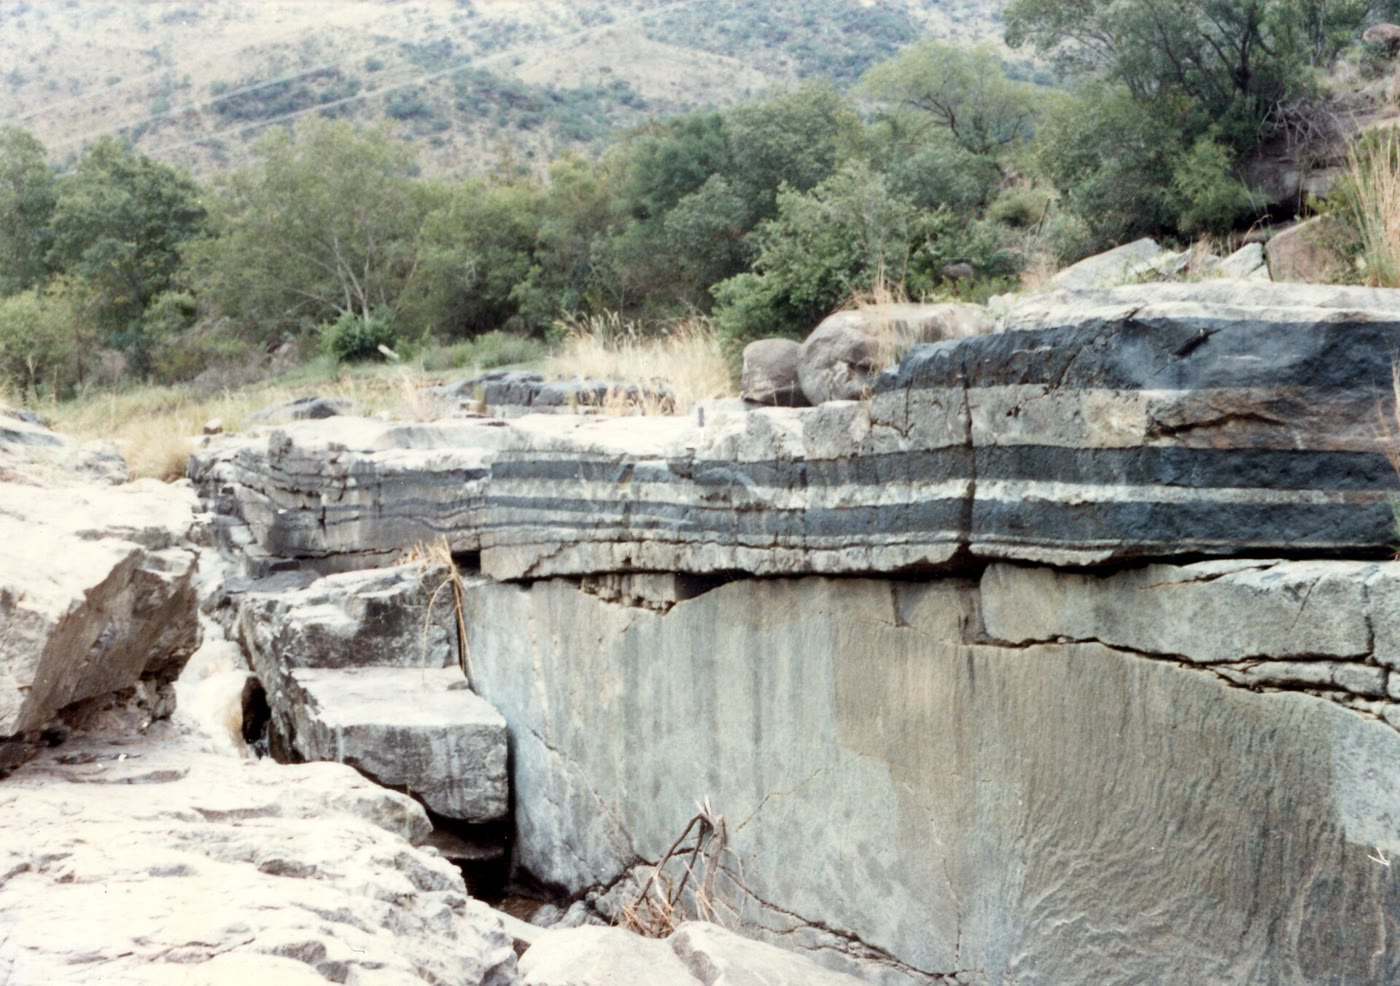
\includegraphics[height=5.2cm]{images/book4/b2-bushveld-chromitite.jpg}
\end{minipage}\hfill
\begin{minipage}[t]{0.42\linewidth}\vspace{0pt}\centering
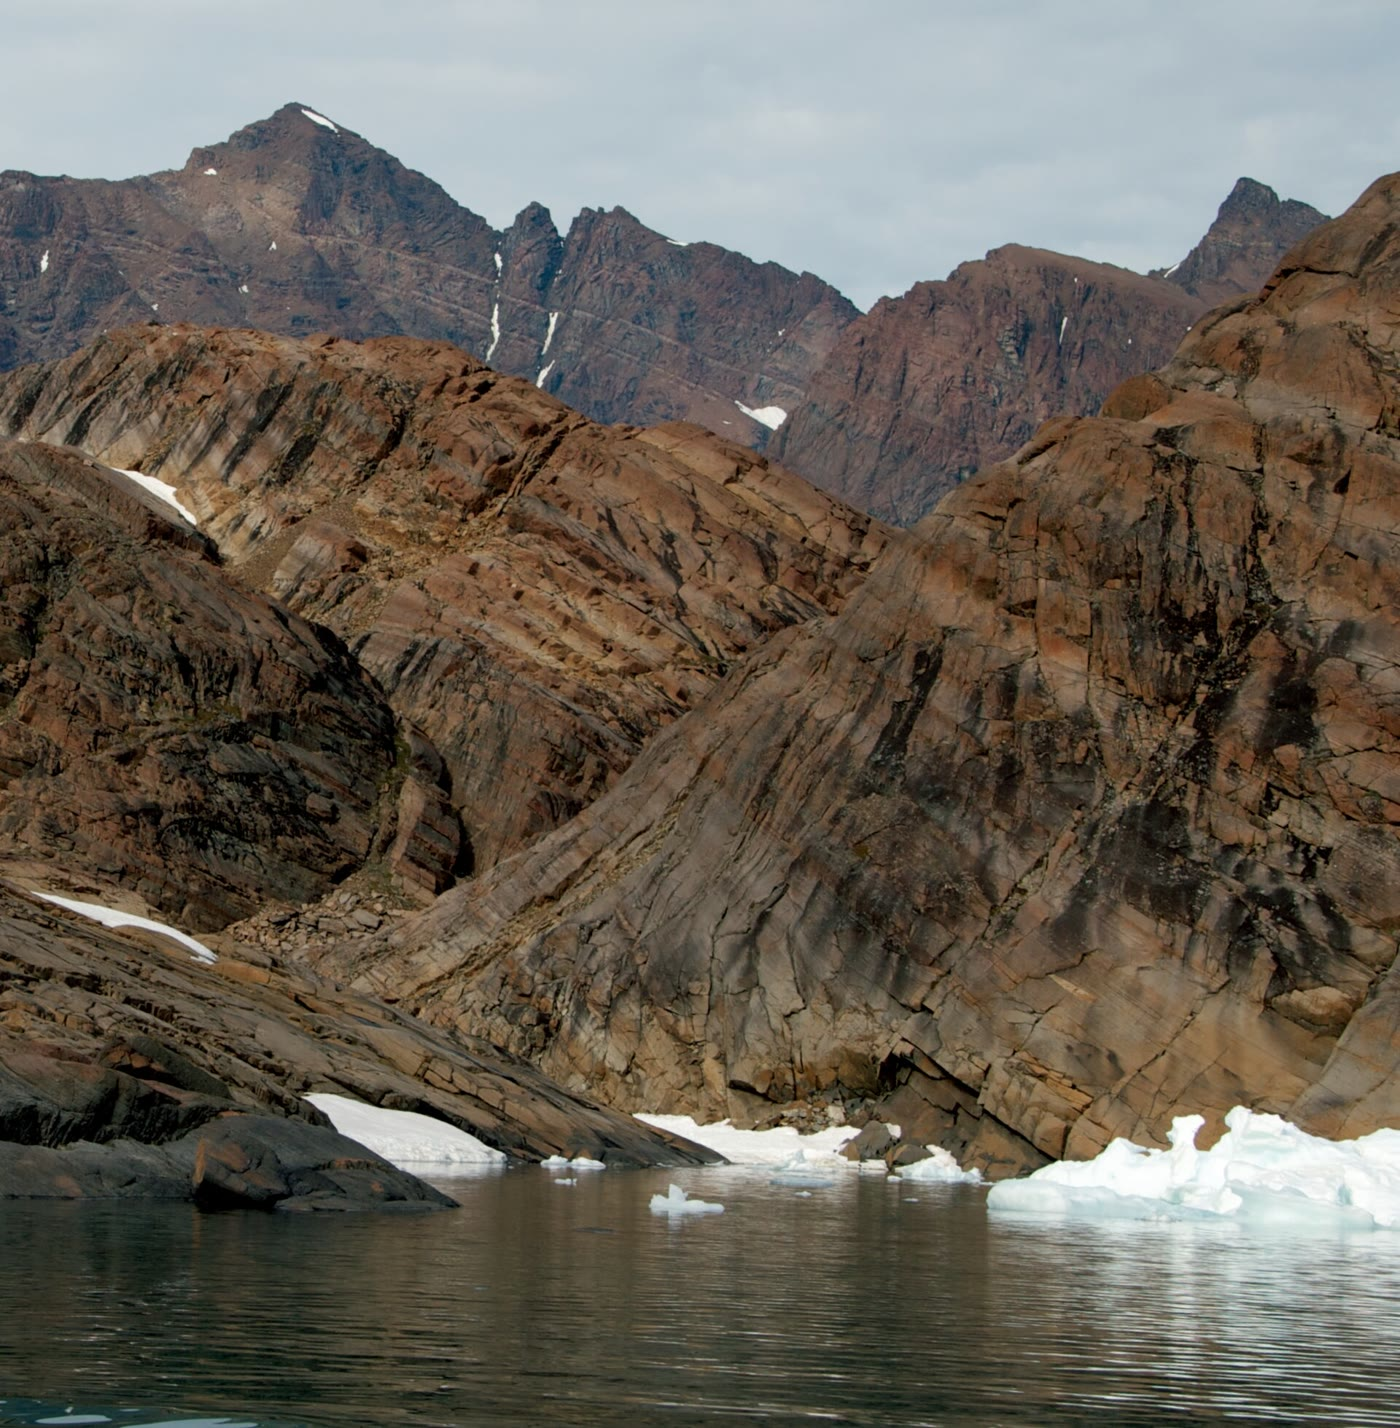
\includegraphics[height=5.2cm]{images/book4/b2-skaergaard-layering.jpg}
\end{minipage}
\par\smallskip{\small اليمين: طبقات الكروميتيت السوداء والأنورثوزيت الرمادي في
المنطقة الحرجة لمعقّد بوشفيلد، جنوب أفريقيا \mbox{\textdir TLT (Kevin Walsh, CC BY 2.0)}.
اليسار: صخور الغابرو الطبقية في المنطقة الوسطى لمتداخل سكيرغارد، شرق
غرينلاند، مائلةً من أعلى اليسار إلى أسفل اليمين \mbox{\textdir TLT (C. Tegner, CC BY 4.0)}.}
\end{omfigure}

\section{الأنظمة المفتوحة}\label{sec:b2:magmatic-differentiation:open}

قلّما تكون الحجرة الصهارية مغلقة. فصهارة جديدة تصل من الأسفل، وجدران
الحجرة صخور تستطيع \omterm{def:b2:magma-emplacement:magma}{الصهارة} أن تسخّنها وتصهرها وتذيبها.

\begin{definition}[امتزاج الصهارات؛ الاستيعاب القشري؛ الاستيعاب مع التبلور التجزيئي]
\label{def:b2:magmatic-differentiation:open}
\emph{امتزاج الصهارات}\index{امتزاج الصهارات} هو خلط صهارتين مختلفتين
تركيبًا في صهارة واحدة. و\emph{الاستيعاب القشري}\index{الاستيعاب القشري} هو
إدخال صخر قشري في صهارة، بصهر صخر الجدار وإذابته
أو صهر كتل سقطت فيها وإذابتها. و\emph{الاستيعاب مع التبلور
التجزيئي}\index{الاستيعاب مع التبلور التجزيئي} \babelsublr{(AFC)} هو
اجتماعهما في حجرة واحدة: تتبلور \omterm{def:b2:magma-emplacement:magma}{الصهارة}، والحرارة الكامنة المتحرّرة
تصهر صخر الجدار وتستوعبه.
\end{definition}

\begin{proposition}[الامتزاج خطي في التراكيز]\label{prop:b2:magmatic-differentiation:mixing}
مزيج من كسر كتلي $s$ من \omterm{def:b2:magma-emplacement:magma}{الصهارة} A و$1-s$ من \omterm{def:b2:magma-emplacement:magma}{الصهارة} B يكون لكل
تركيز فيه $C = sC_A + (1-s)C_B$: ففي أيّ مخطّط لتركيز بدلالة
آخر، تقع المزائج على القطعة المستقيمة من A إلى B، وتعطي قاعدة الرافعة
$s$.
\end{proposition}

\begin{proof}
كل عنصر محفوظ: $C(m_A + m_B) = m_AC_A + m_BC_B$؛ اقسم على $m_A + m_B$.
\end{proof}

الامتزاج وإزالة البلّورات كلاهما يرسم خطوطًا مستقيمة في \omterm{def:b2:magmatic-differentiation:harker}{مخطّطات هاركر}؛ أمّا النسب
النظائرية فتميّز بينهما. فالتبلور لا يغيّر النسبة النظائرية، في حين
يغيّرها الامتزاج بصخر ذي نسبة مختلفة، على امتداد القطع الزائد في
\cref{ch:b2:isotope-geochemistry}. فارتفاع \babelsublr{$^{87}$Sr/$^{86}$Sr} مع السيليكا في
متتالية بركانية هو إذن علامة الاستيعاب.

\begin{proposition}[الاستيعاب مع التبلور التجزيئي]
\label{prop:b2:magmatic-differentiation:afc}
صهارة تبلور بلّورات معامل توزيعها الكلي $D$ لعنصر ما
وتستوعب صخر جدار تركيزه $C_a$ بمعدل يساوي $r$ ضعف معدل
التبلور ($r \ne 1$). فإذا كانت $F$ كتلة \omterm{def:b2:magma-emplacement:magma}{الصهارة} نسبةً إلى كتلتها
الابتدائية و$z = (r + D - 1)/(r - 1)$، فإن
\[
\frac{C}{C_0} = F^{-z} + \frac{r}{r - 1 + D}\,\frac{C_a}{C_0}\,\bigl(1 - F^{-z}\bigr).
\]
ومن أجل $r = 0$ هذا هو قانون رايلي. والنسبة النظائرية للعنصر في \omterm{def:b2:magma-emplacement:magma}{الصهارة}
هي متوسط نسبة \omterm{def:b2:magma-emplacement:magma}{الصهارة} الابتدائية ونسبة صخر الجدار، مرجّحًا
بحدّي هذا المجموع.
\end{proposition}

\begin{proof}
لكل وحدة كتلة ابتدائية، حين تتبلور كتلة $\mathrm dm_c$، تُستوعَب كتلة
$r\,\mathrm dm_c$ وتتغيّر كتلة \omterm{def:b2:magma-emplacement:magma}{الصهارة} بمقدار $\mathrm dM =
-(1-r)\,\mathrm dm_c$. وموازنة العنصر هي $\mathrm d(MC) = rC_a\,\mathrm dm_c -
DC\,\mathrm dm_c$. وبنشر الطرف الأيسر واستبدال $\mathrm dm_c$ بالمقدار
$-\mathrm dM/(1-r)$،
\[
M\frac{\mathrm dC}{\mathrm dM} = -C - \frac{rC_a - DC}{1-r}
= \frac{(r - 1 + D)\,C - rC_a}{1 - r} = -z\,\bigl(C - C^*\bigr),
\qquad C^* = \frac{rC_a}{r - 1 + D}.
\]
إذن $\mathrm d(C - C^*)/(C - C^*) = -z\,\mathrm dM/M$، و$C - C^*$ يتناسب
مع $M^{-z}$؛ ومع $C = C_0$ عند $M = 1$، $C = C^* + (C_0 - C^*)F^{-z}$، وهي
الصيغة. ومن أجل $r = 0$، $z = 1 - D$ و$C^* = 0$. والذرّات الآتية من
\omterm{def:b2:magma-emplacement:magma}{الصهارة} الابتدائية تخضع للمعادلة نفسها مع $C_a = 0$، فتركيزها
$C_0F^{-z}$؛ والباقي يأتي من الجدار: ومن هنا ترجيح النسب النظائرية.
\end{proof}

قدّم دي باولو هذه المعادلات عام 1981، وهي النموذج المعياري لصهارة
تلوّثت في طريقها عبر القشرة. وهي تخفي قيدًا حراريًا. فالحرارة اللازمة
لاستيعاب الصخر تأتي من الحرارة الكامنة للبلّورات: فتسخين القشرة من
150 إلى \qty{1150}{\celsius} يتطلّب نحو \qty{1}{kJ/g}، وصهرها \qty{300}{J/g}،
بينما يعطي تبلور \omterm{def:b2:magma-emplacement:magma}{الصهارة} نحو \qty{400}{J/g}؛ فلا بدّ أن يتبلور نحو \qty{3.25}{g} من
\omterm{def:b2:magma-emplacement:magma}{الصهارة} لكل غرام من الصخر المُستوعَب، و$r$ أدنى من 1 بكثير.
وقد أجرى ويلكوكس الحساب نفسه لباريكوتين: فكتلته البالغة \qty{25.4}{g} من المونزونيت
الكوارتزي، المأخوذة عند نحو \qty{200}{\celsius}، احتاجت إلى نحو \qty{31350}{J} لكي
تُسخَّن إلى \qty{1100}{\celsius} وتنصهر، وهي حرارة تبلور نحو
\qty{85}{g} من البلاجيوكليز، أي أكثر بكثير من \qty{12.5}{g} من البلّورات التي أزالتها
موازنته الكتلية. \omterm{def:b2:magma-emplacement:magma}{فالصهارة} الثائرة لم يكن بوسعها أن تدفع ثمن استيعابها بنفسها:
فلا بدّ أن الحرارة جاءت من جسم صهاري أكبر من الذي ثار،
يتبلور بعيدًا عن الأنظار (\cref{exo:b2:magmatic-differentiation:11}).
% ledger: depaolo81:afc, white09:afc-heat, wilcox54:heat, wilcox54:mass-balance

\begin{omfigure}
\centering
\begin{tikzpicture}
\begin{axis}[omrecord, name=left, width=0.47\linewidth, height=5.4cm,
  xmin=0.3, xmax=1, ymin=0.3, ymax=1.05, x dir=reverse,
  xlabel={الصهارة المتبقّية $F$}, ylabel={\mbox{\textdir TLT Sr: $C/C_0$}},
  tick label style={font=\scriptsize}, label style={font=\small}]
\addplot[thick, black] table[x=F, y=srC_r0] {figdata/out/bachelor-2-differentiation-afc.dat};
\addplot[thick, blue!70!black] table[x=F, y=srC_r02] {figdata/out/bachelor-2-differentiation-afc.dat};
\addplot[thick, red!70!black] table[x=F, y=srC_r05] {figdata/out/bachelor-2-differentiation-afc.dat};
\end{axis}
\begin{axis}[omrecord, at={(left.east)}, anchor=west, xshift=1.7cm,
  width=0.47\linewidth, height=5.4cm,
  xmin=0.3, xmax=1, ymin=0.703, ymax=0.716, x dir=reverse,
  xlabel={الصهارة المتبقّية $F$}, ylabel={\mbox{\textdir TLT $^{87}$Sr/$^{86}$Sr}},
  y tick label style={/pgf/number format/fixed, /pgf/number format/precision=3},
  legend style={font=\scriptsize, at={(0.03,0.97)}, anchor=north west},
  tick label style={font=\scriptsize}, label style={font=\small}]
\addplot[thick, black] table[x=F, y=iso_r0] {figdata/out/bachelor-2-differentiation-afc.dat};
\addlegendentry{$r = 0$}
\addplot[thick, blue!70!black] table[x=F, y=iso_r02] {figdata/out/bachelor-2-differentiation-afc.dat};
\addlegendentry{$r = 0.2$}
\addplot[thick, red!70!black] table[x=F, y=iso_r05] {figdata/out/bachelor-2-differentiation-afc.dat};
\addlegendentry{$r = 0.5$}
\end{axis}
\end{tikzpicture}
\par\smallskip{\small \omterm{def:b2:magmatic-differentiation:open}{الاستيعاب مع التبلور التجزيئي} للسترونشيوم
($D = 1.5$، وصخر جدار فيه نصف سترونشيوم \omterm{def:b2:magma-emplacement:magma}{الصهارة}
و\mbox{\textdir TLT $^{87}$Sr/$^{86}$Sr = 0.7200}، \omterm{def:b2:magma-emplacement:magma}{والصهارة} 0.7035؛ قيم توضيحية). اليسار:
ينخفض التركيز أسرع كلما ارتفع معدل الاستيعاب $r$، لأن صخر الجدار يجلب
سترونشيومًا أقل وتتكوّن بلّورات أكثر من أجل $F$ نفسه. اليمين: النسبة
النظائرية، التي لا يغيّرها التبلور وحده ($r = 0$)، تصعد نحو نسبة الجدار.}
\end{omfigure}

\section{قراءة البلّورات المنطّقة}\label{sec:b2:magmatic-differentiation:zoning}

\begin{definition}[التنطّق التركيبي]\label{def:b2:magmatic-differentiation:zoning}
تُظهر بلّورة محلول صلب \emph{تنطّقًا تركيبيًا}\index{التنطّق التركيبي} حين يتغيّر تركيبها من اللبّ إلى الحافة، مسجّلةً السائل المتغيّر
الذي نمت منه طبقاتها المتعاقبة. ويكون التنطّق \emph{عاديًا} حين تكون الحافة أغنى
بالمكوّن المنخفض الحرارة (الصوديوم في البلاجيوكليز)، و\emph{معكوسًا} حين تكون
أغنى بالمكوّن المرتفع الحرارة، و\emph{تذبذبيًا} حين يتناوبان.
\end{definition}

البلّورة المنطّقة تبلور تجزيئي مضبوط بالجرم المشهود: فلبّها لم
يُعِد توازنه مع السائل اللاحق. ويحسب الشكل أدناه، على حلقة بوين،
البلاجيوكليز النامي من سائل فيه \qty{50}{\percent} من الأنورثيت. ففي
التوازن تبقى البلّورات متجانسة وتنتهي عند \qty{50}{\percent}؛ وفي \omterm{def:b2:magmatic-differentiation:crystallisation}{التبلور
التجزيئي} التام تكون كل طبقة جديدة في توازن مع سائل يزداد غنًى
بالصوديوم، وحافة آخر البلّورات ألبيت شبه نقي. والتنطّق العادي، من
لبّ كلسي إلى حافة صودية، هو ما تتنبّأ به سلسلة بوين لصهارة تبرد. أمّا النطاق
المعكوس، أي شريط كلسي خارج شريط صودي، فيدلّ على أن البلّورة غُمرت فجأة في
سائل أسخن أو أغنى بالكالسيوم: وكثيرًا ما يكون ذلك وصول صهارة جديدة، وامتزاجًا في
الحجرة.
% ledger: bowen13:plagioclase, earle:bowen (Book 2)

\begin{omfigure}
\centering
\begin{tikzpicture}
\begin{axis}[omrecord, width=0.78\linewidth, height=6cm,
  xmin=0, xmax=1, ymin=0, ymax=90,
  xlabel={\foreignlanguage{arabic}{كسر السائل المتبلور}},
  ylabel={\foreignlanguage{arabic}{الأنورثيت \babelsublr{(\unit{\percent})} جزيئيًا}},
  legend style={font=\scriptsize, at={(0.02,0.02)}, anchor=south west},
  tick label style={font=\scriptsize}, label style={font=\small}]
\addplot[very thick, red!70!black] table[x=x, y=an_frac] {figdata/out/bachelor-2-differentiation-zoning.dat};
\addlegendentry{\foreignlanguage{arabic}{التجزيئي: الطبقة المتكوّنة}}
\addplot[thick, gray, densely dotted] table[x=x, y=an_liq_frac] {figdata/out/bachelor-2-differentiation-zoning.dat};
\addlegendentry{\foreignlanguage{arabic}{التجزيئي: السائل}}
\addplot[very thick, blue!70!black, dashed] table[x=x, y=an_eq] {figdata/out/bachelor-2-differentiation-zoning.dat};
\addlegendentry{\foreignlanguage{arabic}{المتوازن: البلّورات}}
\end{axis}
\end{tikzpicture}
\par\smallskip{\small بلاجيوكليز يتبلور من سائل فيه \qty{50}{\percent} من
الأنورثيت، محسوبًا على حلقة بوين (1913). في \omterm{def:b2:magmatic-differentiation:crystallisation}{التبلور التجزيئي} تزداد
الطبقات المتعاقبة للبلّورات، من اللبّ (اليسار) إلى الحافة (اليمين)، غنًى
بالصوديوم، ويبلغ السائل الألبيت حين يتبلور نحو \qty{82}{\percent}؛ وفي
\omterm{def:b2:magmatic-differentiation:crystallisation}{التبلور المتوازن} تبقى البلّورات متجانسة وتنتهي بتركيب
السائل الذي جاءت منه.}
\end{omfigure}

\begin{inthelab}[قراءة البلّورات المنطّقة]
يقرأ علماء الصخور التنطّق أولًا بين مستقطِبين متعامدين، حيث تنطفئ نطاقات
البلاجيوكليز عند زوايا مختلفة قليلًا وتظهر أشرطةً متّحدة المركز.
ثم يقيسونه: فالمسبار الإلكتروني الدقيق (\cref{ch:b2:field-lab-methods-2})
يحلّل بقعًا عرضها بضعة ميكرومترات على امتداد مقطع من اللبّ إلى الحافة، وخرائط
الكالسيوم والصوديوم تُظهر النطاقات مباشرة. ومن هذا المقطع الجانبي يحسبون
تركيب السائل الذي نما منه كل نطاق، بحلقة الشكل أعلاه أو
بمعاملات التوزيع، ويعدّون النطاقات المعكوسة على أنها عدد مرّات
إعادة تغذية الحجرة. والعناصر النزرة المقيسة على المقطع نفسه بالاستئصال
بالليزر، والنسب النظائرية المقيسة نطاقًا نطاقًا، تفصل بين التبلور والامتزاج
والاستيعاب في تاريخ بلّورة واحدة.
\end{inthelab}

\section{التمارين}

\begin{exercise}[$\star$]\label{exo:b2:magmatic-differentiation:1}
استعمل قياسات بوين على البلاجيوكليزات (خط الصلابة ثم خط السيولة، \unit{\celsius}):
An$_{100}$ (1550 و1550)؛ An$_{83.3}$ (1465 و1521)؛ An$_{66.7}$ (1372 و1490)؛ An$_{50}$
(1287 و1450)؛ An$_{33.3}$ (1205 و1394)؛ An$_{20}$ (خط السيولة 1334)؛ An$_{11.1}$ (خط السيولة
1265)، واستكمل خطيًا بين النقاط المتجاورة. يبرد سائل فيه
\qty{50}{\percent} من الأنورثيت في توازن. (أ) عند أيّ درجة حرارة يبدأ
بالتبلور، وما تركيب أول بلّورة؟ (ب) عند
\qty{1394}{\celsius}، ما تركيبا السائل والبلّورات،
وما الكسر الكتلي الذي تبلور (استعمل الكسور المولية كأنها كسور
كتلية)؟ (ج) ما تركيب آخر قطرة من السائل؟
\end{exercise}
% ledger: bowen13:plagioclase

\begin{exercise}[$\star$]\label{exo:b2:magmatic-differentiation:2}
متراكم غابروي فيه \qty{50}{\percent} من البلاجيوكليز، و\qty{35}{\percent} من
الكلينوبيروكسين و\qty{15}{\percent} من الأوليفين. مع معاملات التوزيع
(الأوليفين ثم الكلينوبيروكسين ثم البلاجيوكليز)، للسترونشيوم 0.000063 و0.157 و2.7، وللزركونيوم 0.00068
و0.195 و0.001، وللروبيديوم 0.000044 و0.0033 و0.025، احسب معامل التوزيع
الكلي لكل عنصر، وقل أيّها متوافق.
\end{exercise}
% ledger: white07:kd-basalt

\begin{exercise}[$\star$]\label{exo:b2:magmatic-differentiation:3}
يتبلور متراكم \cref{exo:b2:magmatic-differentiation:2} من بازلت، \omterm{def:b2:magmatic-differentiation:crystallisation}{بالتبلور التجزيئي}،
حتى يبقى نصف السائل. (أ) بأيّ عامل تغيّر كلٌّ من Sr وZr وRb
في السائل (خذ المعاملات الكلية 1.40 و0.069 و0.014)؟ (ب) بأيّ عامل
تغيّرت النسبة Zr/Rb؟ علّق مستعينًا بالنتيجة المتعلّقة بالنسب.
\end{exercise}
% ledger: white07:kd-basalt

\begin{exercise}[$\star$]\label{exo:b2:magmatic-differentiation:4}
كان في أول حمم باريكوتين (فبراير 1943) \qty{55.04}{\percent} من \ce{SiO2}،
و\qty{5.68}{\percent} من \ce{MgO} و\qty{0.85}{\percent} من \ce{K2O}؛ وفي آخرها (فبراير
1952)، 60.07 و3.73 و\qty{1.67}{\percent}. (أ) احسب تغيّر كل أكسيد.
(ب) لا يدخل البوتاس أيًّا من المعادن المتبلورة. فلو كان قد تركّز
\omterm{def:b2:magmatic-differentiation:crystallisation}{بالتبلور التجزيئي} وحده، فما كسر السائل الذي كان سيبقى؟
(ج) لا تزيل الموازنة الكتلية لويلكوكس إلا نحو \qty{12.5}{g} من البلّورات لكل
\qty{100}{g} من \omterm{def:b2:magma-emplacement:magma}{الصهارة}. ماذا توحي المقارنة؟
\end{exercise}
% ledger: wilcox54:table2, wilcox54:mass-balance

\begin{exercise}[$\star\star$]\label{exo:b2:magmatic-differentiation:5}
قارن \omterm{def:b2:magmatic-differentiation:crystallisation}{التبلور التجزيئي} \omterm{def:b2:magmatic-differentiation:crystallisation}{بالتبلور المتوازن}: احسب $C_L/C_0$ بالقانونين
(أ) للنيكل، $D = 5$، حين يتبلور \qty{20}{\percent} من السائل؛ (ب)
لعنصر غير متوافق، $D = 0.01$، حين يتبلور \qty{90}{\percent}.
(ج) ما نهايتا القانونين حين $F \to 0$؟ وأيّ القانونين يستطيع تجريد سائل من
عنصر متوافق تجريدًا تامًا؟
\end{exercise}

\begin{exercise}[$\star\star$]\label{exo:b2:magmatic-differentiation:6}
(أ) احسب النسب المئوية الكتلية لأكاسيد \ce{MgO} و\ce{FeO} و\ce{SiO2} في أوليفين
Fo$_{80}$، $(\ce{Mg}_{0.8}\ce{Fe}_{0.2})_2\ce{SiO4}$ (قيم $M$ هي 40.30 و71.84
و\qty{60.08}{g/mol}). (ب) بازلت فيه \qty{10.0}{\percent} من \ce{MgO}
و\qty{49.0}{\percent} من \ce{SiO2} لا يبلور إلا هذا الأوليفين حتى يصير في سائله
\qty{8.0}{\percent} من \ce{MgO}. ما الكسر الكتلي للأوليفين المُزال؟ (ج) ما
محتوى السائل من السيليكا عندئذ؟
\end{exercise}

\begin{exercise}[$\star\star$]\label{exo:b2:magmatic-differentiation:7}
في متداخل سكيرغارد، $F = \num{1.091e-7}H^2 - \num{5.9064e-4}H + 0.7678$.
(أ) احسب $F$ عند $H = 0$ و1000 و\qty{2000}{m}. (ب) عند أيّ ارتفاع تكون $F = 0$؟
(ج) ما كسر \omterm{def:b2:magma-emplacement:magma}{الصهارة} الذي كان قد تبلور قبل أن تتكوّن قاعدة تتابع الأرضية
المتكشّف، وأين يمكن أن يكون؟
\end{exercise}
% ledger: tegner23:skaergaard

\begin{exercise}[$\star\star$]\label{exo:b2:magmatic-differentiation:8}
على امتداد مقطع سكيرغارد، يحوي \omterm{def:b2:magmatic-differentiation:cumulate}{المتراكم} الوسيط \qty{177}{ppm} من النيكل عند
$F = 0.70$ (الجزء a من المنطقة الدنيا)، و\qty{54}{ppm} عند $F = 0.29$ (المنطقة الوسطى)
و\qty{6.2}{ppm} عند $F = 0.17$ (الجزء a من المنطقة العليا). (أ) بافتراض أن المتراكمات تحوي
$D$ ضعف نيكل سائلها وأن السائل يتبع قانون رايلي،
احسب $D$ الظاهري بين المستويين الأولين. (ب) افعل الشيء نفسه بين
المستويين الأخيرين. (ج) ما الذي يمكن أن يغيّر $D$ الظاهري؟
\end{exercise}
% ledger: data:b4-skaergaard

\begin{exercise}[$\star\star$]\label{exo:b2:magmatic-differentiation:9}
تحقّق من جواب ويلكوكس: \qty{100}{g} من أرضية الحمم الأولى (\ce{SiO2}
55.53، \ce{MgO} 4.66، \ce{K2O} \qty{0.88}{\percent}) زائد \qty{25.4}{g} من متوسط
الصخر الدخيل (72.48، 0.77، 3.64) ناقص \qty{2.9}{g} من أوليفين Fo$_{80}$ (39.19، 42.06، 0)
ناقص \qty{9.6}{g} من بلاجيوكليز An$_{70}$ (50.54، 0، 0). (أ) ما الكتلة الباقية؟
(ب) احسب ما فيها من \ce{SiO2} و\ce{MgO} و\ce{K2O} وقارنه بأرضية
الحمم 19 (60.16 و3.19 و\qty{1.75}{\percent}). (ج) أيّ أكسيد يلائم أسوأ ملاءمة؟
\end{exercise}
% ledger: wilcox54:groundmass, wilcox54:xenoliths, wilcox54:mass-balance

\begin{exercise}[$\star\star\star$]\label{exo:b2:magmatic-differentiation:10}
تستوعب صهارة صخر الجدار بالمعدل $r = 0.2$ وهي تتبلور، مع $D_{\ce{Sr}} =
1.5$، $C_a/C_0 = 0.5$، والنسبة الابتدائية \mbox{\textdir TLT $^{87}$Sr/$^{86}$Sr = 0.7035} ونسبة صخر الجدار 0.7200.
(أ) احسب $z$ و$F^{-z}$ و$C/C_0$ عند $F = 0.7$. (ب) قارن \omterm{def:b2:magmatic-differentiation:crystallisation}{بالتبلور التجزيئي}
الخالص عند $F$ نفسه، وفسّر الفرق بكتلة البلّورات
المتكوّنة في كل حالة. (ج) احسب النسبة \babelsublr{$^{87}$Sr/$^{86}$Sr} للصهارة.
\end{exercise}

\begin{exercise}[$\star\star\star$]\label{exo:b2:magmatic-differentiation:11}
تتبّع الموازنة الحرارية لويلكوكس في باريكوتين. (أ) كم من الحرارة يحتاج غرام من
المونزونيت الكوارتزي لينتقل من 200 إلى \qty{1100}{\celsius} (السعة الحرارية
\qty{1.1}{J/(g.K)}) ثم لينصهر (\qty{250}{J/g})؟ (ب) وكم من أجل
\qty{25.4}{g}؟ (ج) ما كتلة البلاجيوكليز An$_{70}$ (حرارته الكامنة \qty{370}{J/g})
التي يجب أن تتبلور لتوفيرها؟ (د) قارن بكتلة البلّورات البالغة \qty{12.5}{g} في
الموازنة الكتلية، واحسب النسبة $r$ بين الاستيعاب والتبلور، وقل ماذا
يقتضي ذلك.
\end{exercise}
% ledger: wilcox54:heat, white09:afc-heat

\begin{exercise}[$\star\star\star$]\label{exo:b2:magmatic-differentiation:12}
بازلت فيه \qty{250}{ppm} من النيكل يبلور أولًا الأوليفين وحده ($D = 5$) حتى
$F = 0.8$، ثم الأوليفين مع البلاجيوكليز والكلينوبيروكسين ($D = 1.5$ للمجموعة كلها). (أ)
احسب العامل الذي يتغيّر به النيكل في كل مرحلة، ومحتوى السائل من النيكل
عند $F = 0.5$. (ب) بماذا كان سيتنبّأ قانون واحد مع $D = 5$؟
(ج) اشرح لماذا يجب تطبيق قانون رايلي على مراحل.
\end{exercise}

\section{مسألة: المتداخل الذي كتب تاريخه بنفسه}

\begin{problem}[{مسألة نهاية الأسبوع --- من طبقات غابرو إلى كسر
صهارته الذي بقي سائلًا في النهاية}]
\label{pb:b2:magmatic-differentiation:1}
عتبة غابروية طبقية (مختلَقة) تبلورت من بازلت تعطي حافته المبرّدة
تركيب الأمّ: \ce{SiO2} 49.5، \ce{Al2O3} 16.0، \ce{FeO} 10.0،
\ce{MgO} 9.0، \ce{CaO} 11.5، \ce{Na2O} 2.5، \ce{K2O} \qty{0.30}{\percent}؛
و\qty{150}{ppm} من النيكل و\qty{80}{ppm} من الزركونيوم. تتكوّن متراكمات المنطقة الدنيا من
\qty{20}{\percent} من الأوليفين و\qty{50}{\percent} من البلاجيوكليز و\qty{30}{\percent} من
الكلينوبيروكسين؛ وفوق المستوى الذي يختفي عنده الأوليفين، من \qty{55}{\percent} من
البلاجيوكليز و\qty{45}{\percent} من الكلينوبيروكسين. خذ معاملات التوزيع
(الأوليفين ثم البلاجيوكليز ثم الكلينوبيروكسين)، للنيكل 5.0 و0 و2.0، وللزركونيوم 0.0007 و0.001
و0.195. تراكيب المعادن (\unit{\percent}): الأوليفين \ce{MgO} 42.06، \ce{CaO} 0،
\ce{Al2O3} 0، \ce{SiO2} 39.19؛ البلاجيوكليز 0، 14.36، 31.70، 50.54؛ الكلينوبيروكسين
16.0، 20.5، 3.0، 51.5. وقاطع
من صخر دقيق الحبيبات غذّته الحجرة حين تبلورت الطبقة العليا، تركيبه
\ce{SiO2} 50.0، \ce{Al2O3} 14.1، \ce{FeO} 16.7، \ce{MgO} 4.9، \ce{CaO} 7.3،
\ce{Na2O} 3.4، \ce{K2O} \qty{0.75}{\percent} و\qty{188}{ppm} من الزركونيوم.

\noindent\textbf{الجزء الأول --- معاملات توزيع الطبقات.}
\begin{enumerate}
\item احسب معامل التوزيع الكلي للنيكل في المنطقة الدنيا.
\item احسب معامل الزركونيوم في المنطقة الدنيا.
\item احسب المعاملين كليهما في المنطقة العليا.
\item أيّ العنصرين متوافق في كل منطقة؟ وهل يبقى النيكل متوافقًا حين
يختفي الأوليفين؟
\item أيّ معدن يحوي معظم زركونيوم المتراكمات، ولماذا؟
\item بأيّ عامل تتغيّر النسبة Ni/Zr في السائل كلما انتصف $F$ في المنطقة
الدنيا؟
\end{enumerate}

\noindent\textbf{الجزء الثاني --- منحنيات رايلي صعودًا في المقطع.}
\begin{enumerate}[resume]
\item ما محتوى النيكل الذي تتوقّعه في أدنى متراكم، المتبلور عند
$F = 1$؟
\item يحوي متراكم من المنطقة الدنيا أعلى منه \qty{190}{ppm} من النيكل. عند أيّ $F$
تكوّن؟
\item ما كان محتوى السائل من الزركونيوم عندئذ؟
\item عند قيمة $F$ تلك، قارن نيكل السائل الذي يعطيه القانونان التجزيئي
والمتوازن.
\item يختفي الأوليفين عند $F = 0.55$. احسب محتوى السائل من النيكل
هناك.
\item احسب نيكل المتراكمات المتكوّنة تحت ذلك المستوى مباشرة وفوقه مباشرة.
ما المعلم الذي يراه الجيولوجي في المقطع الجانبي؟
\item احسب نيكل السائل \omterm{def:b2:magmatic-differentiation:cumulate}{والمتراكم} عند $F = 0.40$. فسّر
الاتجاه.
\end{enumerate}

\noindent\textbf{الجزء الثالث --- الموازنة الكتلية لآخر سائل.}
\begin{enumerate}[resume]
\item اكتب معادلة الحفظ في الطريقة لأكسيد واحد، مع الكتل
$x_{\mathrm{ol}}, x_{\mathrm{pl}}, x_{\mathrm{cpx}}$ المُزالة لكل \qty{100}{g} من
الأمّ \omterm{def:b2:magma-emplacement:bodies}{والقاطع} بوصفه الوليد.
\item اكتبها لأكاسيد \ce{MgO} و\ce{CaO} و\ce{Al2O3}.
\item حلّ النظام $3 \times 3$.
\item ما الكسر من الأمّ الذي يبقى سائلًا؟
\item تحقّق من الجواب بأكسيد \ce{SiO2}: أعد حساب سيليكا السائل من
الكتل الموجودة.
\item قارن نسب المعادن المُزالة بالتراكيب المعدنية في
المنطقتين.
\item لا يدخل البوتاس أيًّا من المعادن: فما كسر السائل الذي يعطيه؟
\end{enumerate}

\noindent\textbf{الجزء الرابع --- كسر السائل في القمة.}
\begin{enumerate}[resume]
\item بأيّ عامل كان الزركونيوم قد ارتفع في السائل حين اختفى الأوليفين عند
$F = 0.55$؟ أعطِ محتوى الزركونيوم عندئذ.
\item من زركونيوم \omterm{def:b2:magma-emplacement:bodies}{القاطع}، احسب كسر السائل المتبقّي حين
تكوّن، بتطبيق قانون المنطقة العليا ابتداءً من $F = 0.55$.
\item أعد الحساب بقيمة واحدة $D = 0.07$ منذ البداية. هل الجواب
حسّاس لتفاصيل $D$؟
\item ارتفع الحديد من 10.0 إلى \qty{16.7}{\percent} في السائل بينما لم تكد السيليكا
تتغيّر. أيّ المعادن مسؤول عن ذلك، وأيّ نوع من المتتاليات الصهارية
ينذر به هذا (\cref{ch:b2:magmatic-series})؟
\item تحوي المتراكمات العليا \qty{47}{ppm} من الزركونيوم. والبلّورات المتراكمة وحدها تحوي
$\bar D$ ضعف زركونيوم السائل؛ فما الكسر الكتلي للسائل المحبوس
(بتركيب \omterm{def:b2:magma-emplacement:bodies}{القاطع}) الذي يفسّر التحليل؟
\item اذكر كسر \omterm{def:b2:magma-emplacement:magma}{الصهارة} الأصلية الذي كان لا يزال سائلًا حين تبلورت
الطبقة العليا، وهو الرقم الأساسي في هذه المسألة، وقارن التقديرات الثلاثة
(العناصر الرئيسية، البوتاس، الزركونيوم).
\end{enumerate}
\end{problem}
% ledger: white07:kd-basalt, matzen12:dni
